% !TeX program = pdflatex
\documentclass[11pt,a4paper]{article}
\usepackage[utf8]{inputenc}
\usepackage[T1]{fontenc}
\usepackage[turkish]{babel}
\usepackage{lmodern}
\usepackage{geometry}
\usepackage{graphicx}
\usepackage{float}
\usepackage[section]{placeins}
\usepackage{flafter}
\usepackage{caption}
\usepackage{subcaption}
\usepackage{booktabs}
\usepackage{siunitx}
\usepackage{hyperref}
\usepackage{longtable}
\usepackage{xcolor}
\usepackage{microtype}
\usepackage{etoolbox}

\geometry{margin=1.3cm}
\hypersetup{colorlinks=true,linkcolor=blue,citecolor=blue,urlcolor=blue}
\graphicspath{{../results/}}
% Görseller için varsayılan ölçek ve oran koruma
\setkeys{Gin}{width=1\linewidth, keepaspectratio}

% Yüzen nesneleri başlık altında tutmak için sıkı kurallar
\floatplacement{figure}{H}
\floatplacement{table}{H}
\captionsetup{font=small,labelfont=bf}
\preto\section{\FloatBarrier}
\preto\subsection{\FloatBarrier}
\AfterEndEnvironment{figure}{\FloatBarrier}
\AfterEndEnvironment{table}{\FloatBarrier}
\AfterEndEnvironment{longtable}{\FloatBarrier}

\title{NPM Ekosisteminde Yönlü Karmaşık Ağ Analizi}
\author{\textbf{Yusuf Talha ARABACI}}
\date{\today}

\begin{document}
\maketitle

\begin{abstract}
NPM ekosisteminde tek bir bağımlılıktaki kusur veya kötü niyetli değişiklik, transitif bağımlılıklar üzerinden geniş bir etki alanına yayılabilir. Bu rapor, paket içeriklerinden ziyade paketler arası ilişkilerin \emph{topolojik} yapısına odaklanır. Bağımlı $\to$ bağımlılık yönünde kurulan yönlü ağ üzerinde in-degree, out-degree ve betweenness merkeziyetleri hesaplanır; bu ölçüler min--max normalizasyonu ile bir \emph{bileşik risk skoru}na dönüştürülür. Ayrıca, en kritik düğümlerin çıkarılmasıyla ağın bağlanırlığı üzerinden bir \emph{sağlamlık} değerlendirmesi yapılır. Tüm görseller ve tablolar results/ dizinindeki çıktılara dayanır ve ilgili başlıklar altında sunulur.
\end{abstract}

\clearpage

\section{Giriş ve Amaç}
Modern yazılım tedarik zincirinde tek bir bağımlılıktaki hata veya kasıtlı bir saldırı, transitif bağımlılıklar üzerinden yüzlerce hatta binlerce projeye yayılabilir. NPM ekosistemi; büyük ölçek, hızlı sürüm döngüleri ve yoğun bağımlılık grafiği nedeniyle bu tür zincirleme risklere özellikle açıktır. Bu rapor, paket içeriğinden ziyade paketler arası ilişkinin topolojik yapısına odaklanır: Bir paketin ağ içindeki konumu ve bu konumun sistemik etkileri nicel olarak değerlendirilir.

Bu çalışmanın hedefi, NPM bağımlılıklarını yönlü bir ağ olarak modelleyip yapısal riski görünür kılmaktır. Bunun için:
\begin{itemize}
  \item Bağımlı $\to$ bağımlılık yönünde kurulan ağ üzerinde, \emph{omurga} ve \emph{köprü} niteliğindeki paketler merkeziyet ölçütleriyle (in-degree, out-degree, betweenness) belirlenir.
  \item Bu ölçütlerden türetilen \emph{bileşik risk skoru} ile paketler karşılaştırılabilir biçimde sıralanır.
  \item Kritik düğümlerin çıkarılmasına dayalı \emph{sağlamlık} göstergeleriyle (zayıf bileşen sayısı, en büyük bileşen boyutu vb.) ağın kırılganlığı nicel olarak değerlendirilir.
\end{itemize}
Bu yaklaşım, güvenlik değerlendirmesini yalnızca paket içi zafiyetlere indirgemek yerine, bağımlılık topolojisinden kaynaklanan yapısal riskin de hesaba katılmasını sağlar. Böylece bakımı yapılacak, yakından izlenecek veya kısıtlanacak paketler veri temelli biçimde önceliklendirilebilir.

\section{Kuramsal Çerçeve ve Tanımlar}
\textbf{Yönlü Ağ (DiGraph).} Düğümler paketleri, yönlü kenarlar ise ``bağımlı $\to$ bağımlılık'' ilişkisini temsil eder. Bir paketin başka bir paketi \emph{kullanması}, bağımlı paketten bağımlılığa giden bir ok (out-edge) ile modellenir.

\textbf{In-degree.} Bir düğüme \emph{gelen} kenar sayısıdır; başka kaç paket o pakete bağımlıdır. Yüksek in-degree, \emph{yayılım potansiyelini} (tekil bir sorun çok projeyi etkileyebilir) ve \emph{omurga} konumunu işaret eder.

\textbf{Out-degree.} Bir düğümden \emph{çıkan} kenar sayısıdır; paketin kaç bağımlılığı vardır. Yüksek out-degree, \emph{bağımlılık yüzeyinin geniş} olduğunu ve tedarik riskine maruziyetin arttığını gösterir.

\textbf{Betweenness Merkeziyeti.} En kısa yollar üzerinde bir düğümün \emph{köprü} (aracılık) rolünü ölçer. Topolojik \emph{boğaz noktaları}nı belirler; tek hata noktası riski taşıyan düğümleri ortaya çıkarır.

\textbf{Bileşik Risk Skoru.} Normalize edilmiş (min--max) ölçülerin ağırlıklı toplamıdır:
\[\mathrm{risk}(n) = w_{in}\,\tilde d_{in}(n) + w_{out}\,\tilde d_{out}(n) + w_b\,\tilde b(n)\]
Burada $\tilde x = (x - x_{\min})/(x_{\max}-x_{\min})$ min--max normalizasyonudur (payda 0 ise $\tilde x=0$). Ağırlıklar $w_{in}, w_{out}, w_b$, omurga duyarlılığı (in-degree), bağımlılık yüzeyi (out-degree) ve köprü rolü (betweenness) arasında vurguyu dengeler.

\textbf{Sağlamlık (Robustluk) ve Kaskad Etkisi.} Risk sıralamasına göre en kritik $k\in\{1,3,5\}$ düğüm çıkarılır; zayıf bağlanırlık bileşen sayısı, en büyük bileşen boyutu ve (mümkünse) ağ çapı ölçülür. \emph{Kaskad etkisi}, bir düğümdeki sorunun transitif olarak etkileyebileceği paket sayısını ifade eder.

\section{Veri ve Yöntem}
\textbf{Veri Toplama.} Top~N paket listeleri ve bağımlılıklar öncelikle ecosyste.ms API’lerinden; yedek olarak npm registry ve npms.io üzerinden alınır. Varsayılan olarak dependencies alanı kullanılır; isteğe bağlı olarak peerDependencies dahil edilebilir.

\textbf{Ön İşleme.} Paket adları normalize edilir; yinelenen kayıtlar ayıklanır; yönlü kenarlar bağımlı $\to$ bağımlılık yönünde oluşturulur. Sürüm tercihinde en güncel kararlı sürümler esas alınır.

\textbf{Ağın Kurulumu.} NetworkX ile DiGraph kurulup düğümler/kenarlar eklenir. Tüm düğümler için in/out-degree hesaplanır; büyük graflarda betweenness, örnekleme ($k$) ile hızlandırılır (rastgele kaynak düğüm seçimi).

\textbf{Risk Skoru Hesabı.} Ölçüler gözlenen aralıkları üzerinden min--max normalize edilir. Ağırlıklar (ör. $w_{in}=0.5$, $w_{out}=0.2$, $w_b=0.3$) omurga duyarlılığı, bağımlılık yüzeyi ve köprü rolü arasında bir denge sağlar; eşitlik durumunda bağıl sıralama korunur.

\textbf{Sağlamlık Deneyi.} Risk sıralamasındaki ilk $k$ düğüm grafikten kaldırılır; zayıf bileşen sayısı ve en büyük bileşen boyutu raporlanır (robustness\_risk.json). Bu göstergeler, \emph{kritik düğüm kaybına} karşı ağın kırılganlığını nicel olarak özetler.

\textbf{Üretilen Çıktılar.} Görseller ve tablolar results/ altında saklanır: ağ görselleri, derece histogramları ve saçılım grafikleri, merkeziyet liderleri, risk sıralaması, kaskad etkisi ve özet metrik tabloları.

\section{Bulgular ve Yorum}
Bu bölümde, results/ dizininden seçilen görseller/tablolar sunulur ve her biri doğrudan altında yorumlanır.

\subsection{Ağın Genel Görünümü}
\begin{figure}[H]
  \centering
  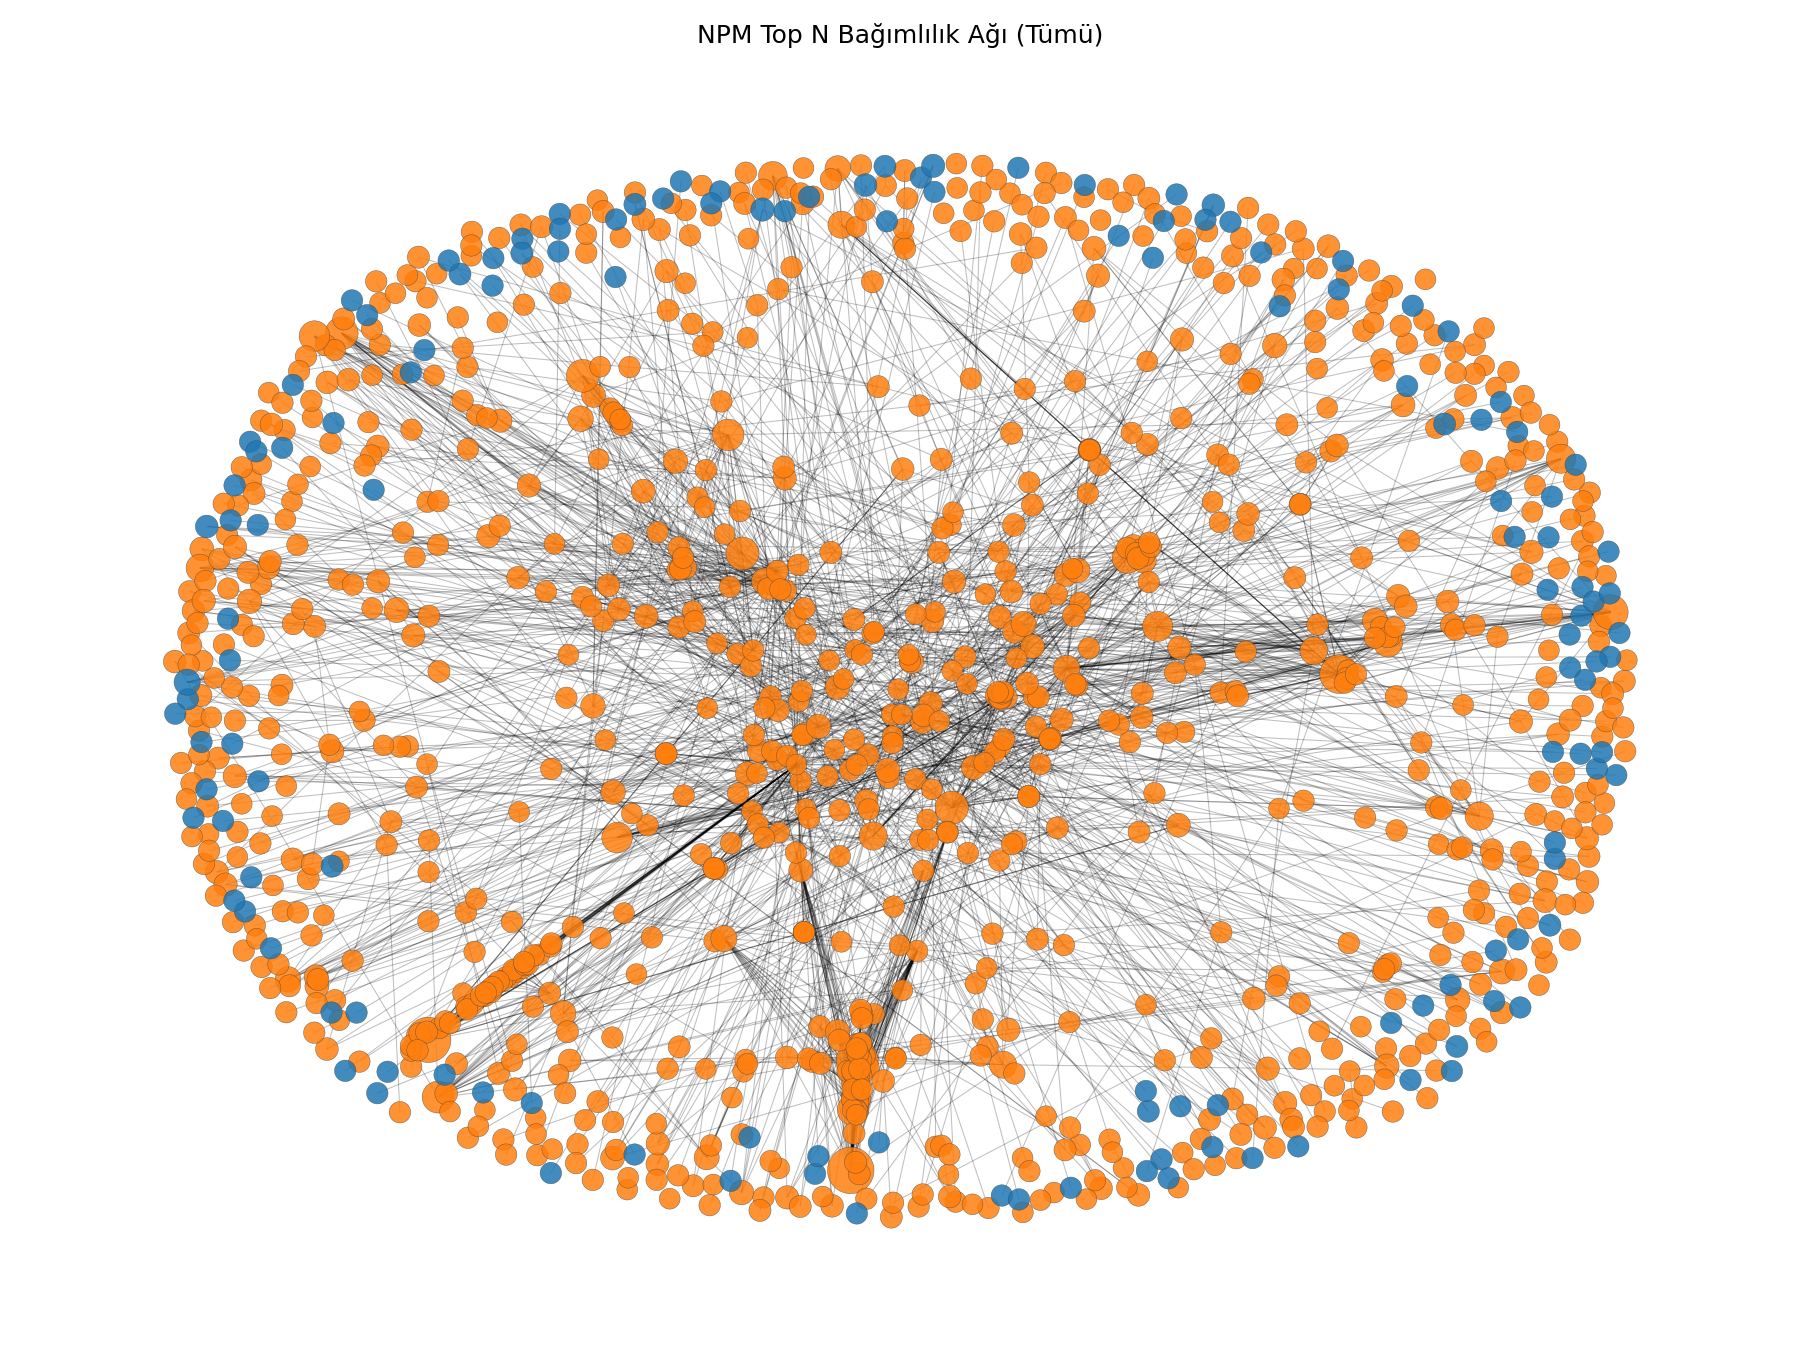
\includegraphics{network_full_topN.png}
  \caption{Top~N ve bağımlılıklarının oluşturduğu yönlü ağ. Düğüm boyutu in-degree ile, renkler Top~N (turuncu) ve diğerleri (mavi) olarak kodlanmıştır. Yüksek in-degree’li düğümler ekosistemin omurgasını oluşturur; bu düğümlerdeki sorunlar geniş yayılıma neden olabilir.}
\end{figure}

\noindent Görsel, merkezî kümelenmeleri ve omurga düğümleri ayırt etmeyi kolaylaştırır. Düğümler arası yoğun bölgeler, paket ekosistemindeki birlikte-kullanım kalıplarına işaret eder.

\begin{figure}[H]
  \centering
  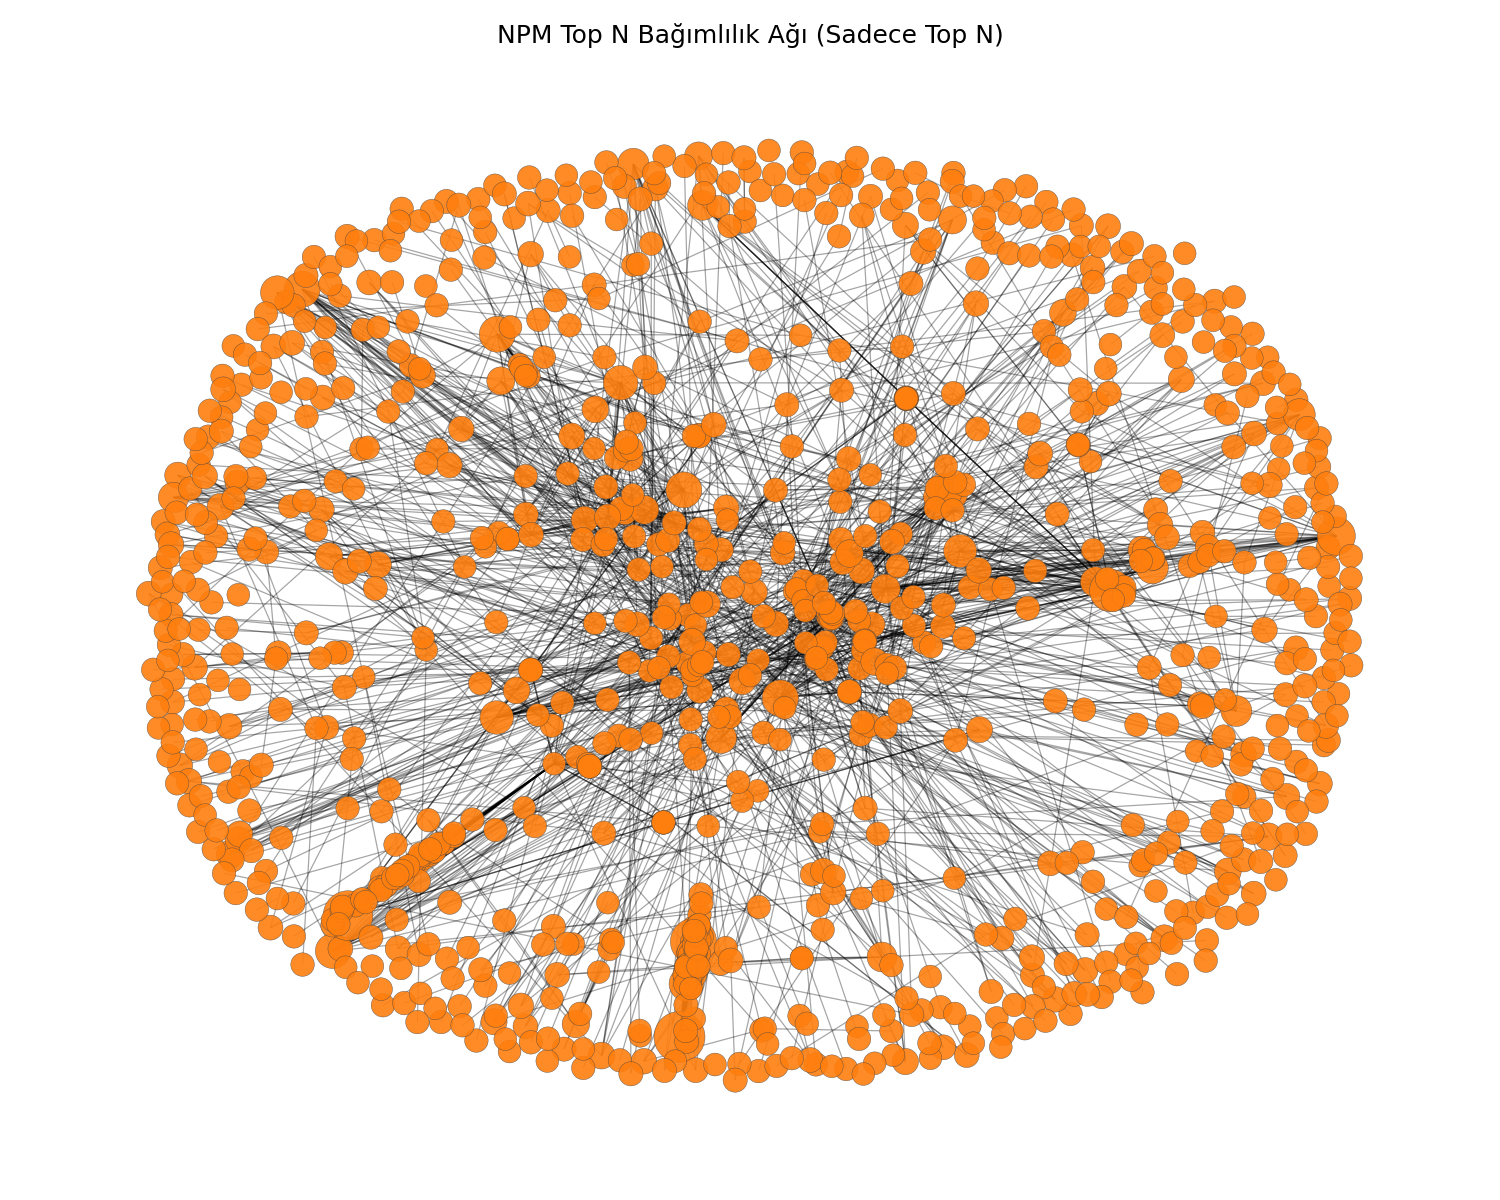
\includegraphics{network_topN_only.png}
  \caption{Sadece Top~N düğümlerin indüklenmiş alt-ağı. Paketin ağ içi konumuna göre merkezî (yüksek in-degree/betweenness) düğümler görselde öne çıkar.}
\end{figure}

\noindent Top~N alt-ağında bağlantı motifleri daha belirgindir. Zincirleme etkinin Top~N içinde nasıl yayılabileceği niteliksel olarak gözlemlenebilir.

\subsection{Derece Dağılımları ve İlişkiler}
\begin{figure}[H]
  \centering
  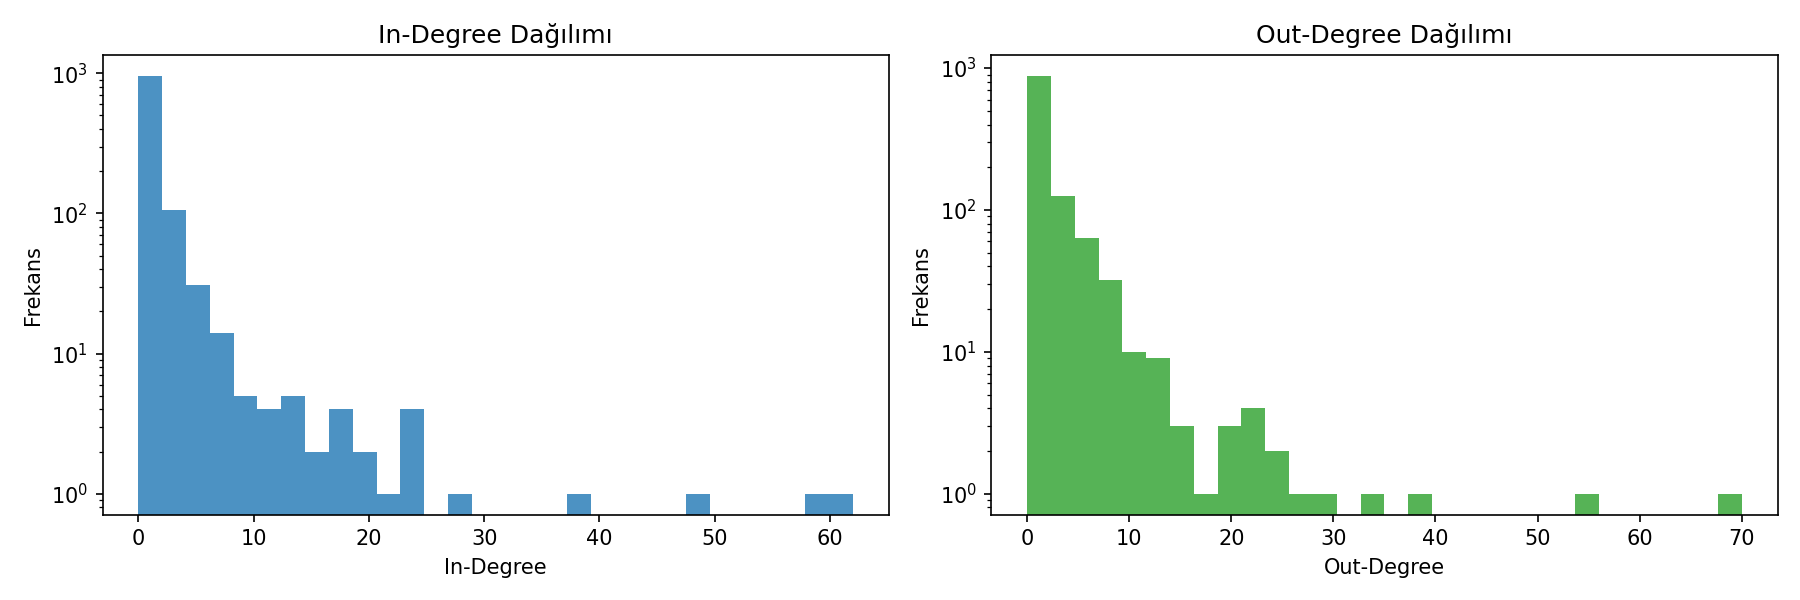
\includegraphics{degree_histograms.png}
  \caption{In-degree ve out-degree histogramları (log ölçek). Ağın ağır kuyruklu yapısı, az sayıda çok etkili paket ile çok sayıda düşük dereceye sahip paketin birlikte varlığını gösterir.}
\end{figure}

\noindent In-degree dağılımı, sistemik etkisi yüksek omurga paketlerini az sayıda düğümde toplar. Out-degree dağılımı, bazı paketlerin geniş bağımlılık yüzeyi nedeniyle tedarik riskine daha açık olduğunu gösterir.

\begin{figure}[H]
  \centering
  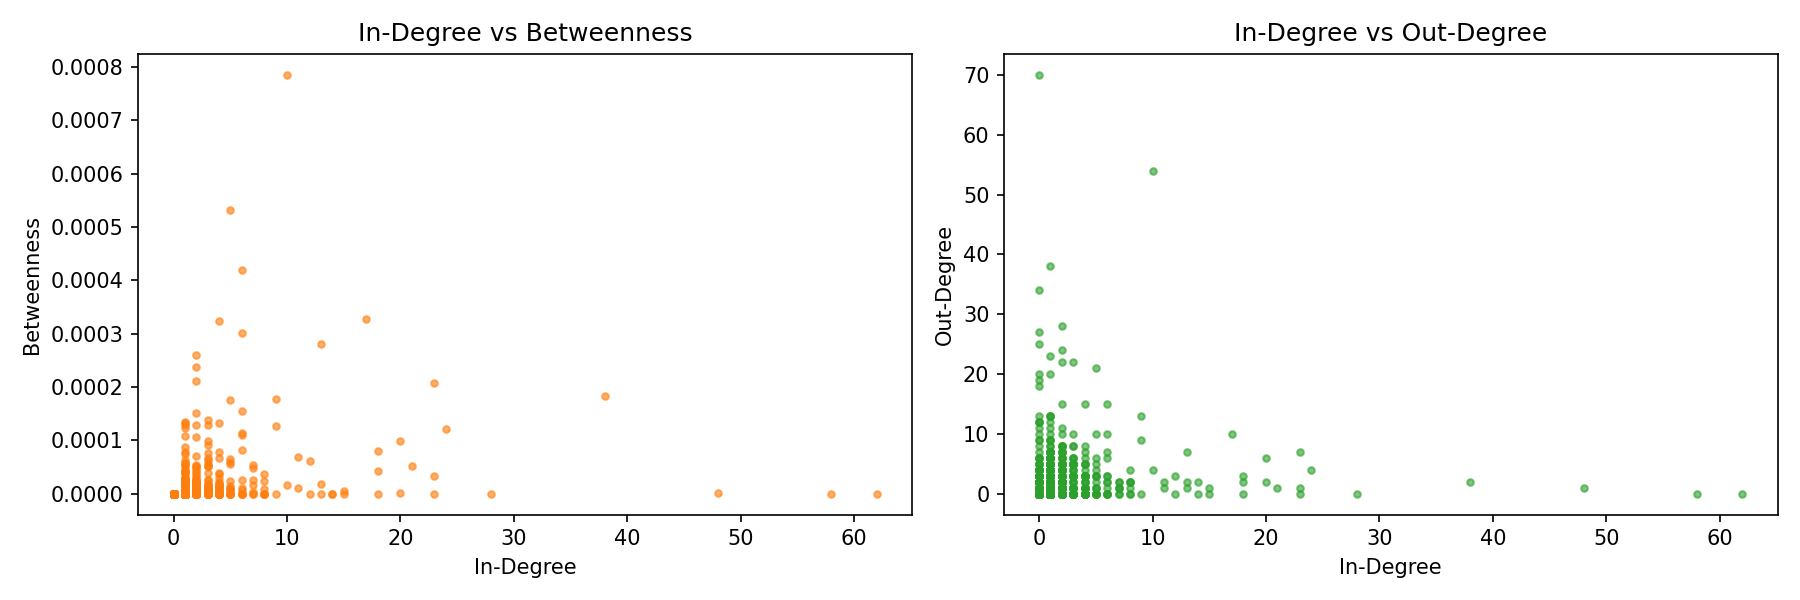
\includegraphics{scatter_correlations.png}
  \caption{Korelasyonlar: (sol) In-degree vs Betweenness; (sağ) In-degree vs Out-degree. In-degree ile betweenness arasındaki pozitif ilişki, omurga düğümlerin çoğu zaman köprü rolünde olduğunu gösterir.}
\end{figure}

\noindent In-degree ile out-degree ilişkisi, bir paketin hem çok kullanılıyor hem de çok sayıda bağımlılığa sahip olabildiğini; bu durumda hem yayılım hem maruziyet riskinin birlikte arttığını gösterir.

\subsection{Merkeziyet Liderleri}
\begin{figure}[H]
  \centering
  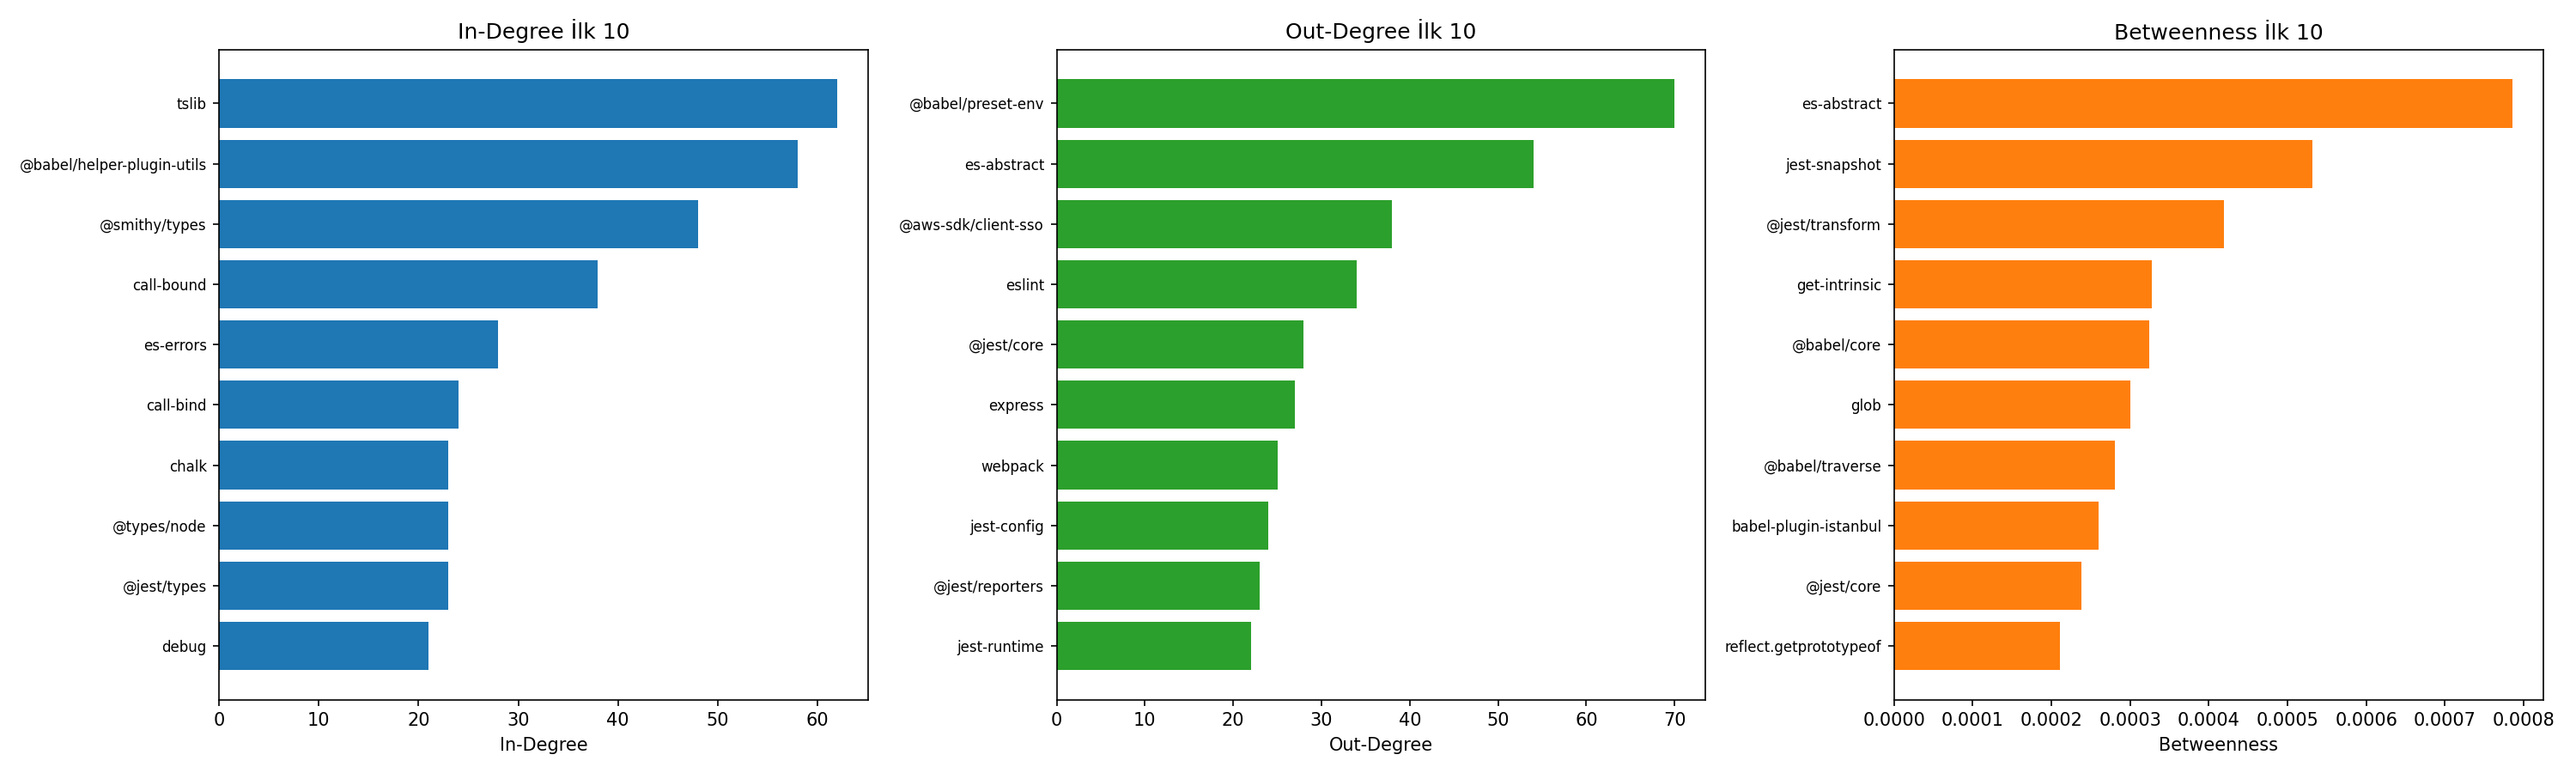
\includegraphics{top10_leaders.png}
  \caption{Merkeziyet liderleri (ilk 10): In-degree, Out-degree ve Betweenness karşılaştırması tek görselde. In-degree liderleri yayılım etkisi yüksek paketleri; Out-degree liderleri geniş bağımlılık yüzeyini; yüksek Betweenness ise köprü/boğaz noktası riskini gösterir.}
\end{figure}

\noindent Bir arada sunulan liderlik çizelgeleri, yayılım (in-degree), maruziyet (out-degree) ve köprü (betweenness) etkilerini aynı anda okumayı kolaylaştırır.

\subsection{Bileşik Risk Skoru}
\begin{figure}[H]
  \centering
  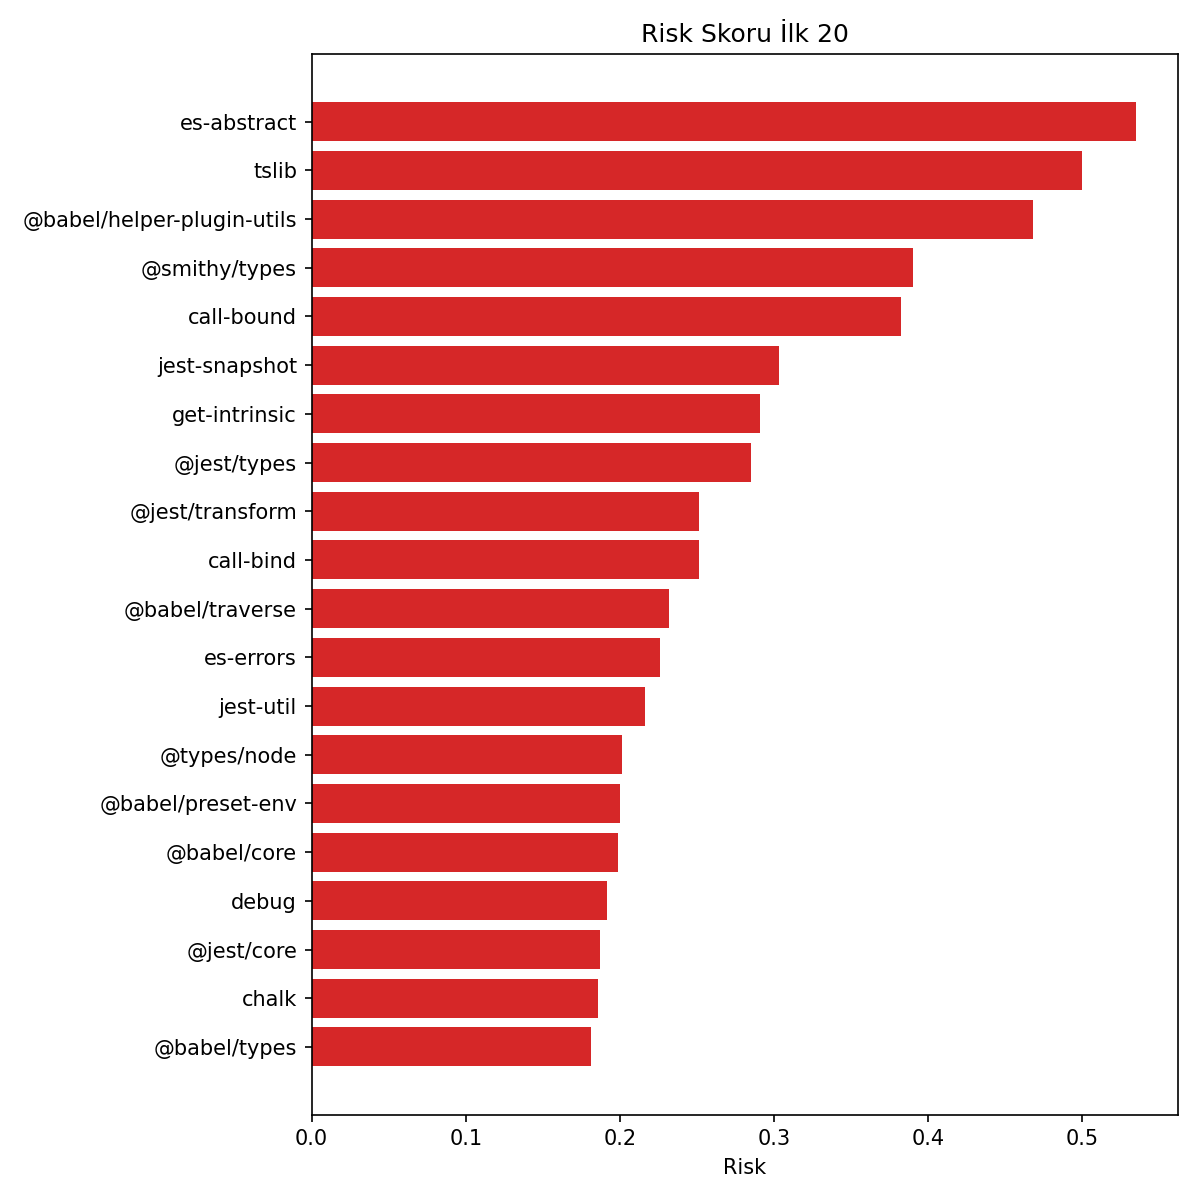
\includegraphics{top20_risk.png}
  \caption{Bileşik risk skoru ile en riskli 20 paket. Ağırlıklar in/out/betweenness arasında denge kuracak biçimde seçilmiştir.}
\end{figure}
\IfFileExists{../results/risk_scores_top20.tex}{\begin{longtable}{lrrrrr}
\caption{Top 20 Risk Skoru}\\
\toprule
Paket & Risk & In-Degree & Out-Degree & Betweenness & TopN? \\
\midrule
\endfirsthead
\toprule
Paket & Risk & In-Degree & Out-Degree & Betweenness & TopN? \\
\midrule
\endhead
\bottomrule
\endfoot
\bottomrule
\endlastfoot
es-abstract & 0.534931 & 10 & 54 & 0.000785 & True \\
tslib & 0.500000 & 62 & 0 & 0.000000 & True \\
@babel/helper-plugin-utils & 0.467742 & 58 & 0 & 0.000000 & True \\
@smithy/types & 0.390249 & 48 & 1 & 0.000001 & True \\
call-bound & 0.382129 & 38 & 2 & 0.000183 & True \\
jest-snapshot & 0.303511 & 5 & 21 & 0.000532 & True \\
get-intrinsic & 0.290993 & 17 & 10 & 0.000328 & True \\
@jest/types & 0.284735 & 23 & 7 & 0.000207 & True \\
@jest/transform & 0.251456 & 6 & 15 & 0.000419 & True \\
call-bind & 0.251171 & 24 & 4 & 0.000121 & True \\
@babel/traverse & 0.231984 & 13 & 7 & 0.000280 & True \\
es-errors & 0.225806 & 28 & 0 & 0.000000 & True \\
jest-util & 0.216164 & 20 & 6 & 0.000099 & True \\
@types/node & 0.201331 & 23 & 1 & 0.000034 & True \\
@babel/preset-env & 0.200000 & 0 & 70 & 0.000000 & True \\
@babel/core & 0.199075 & 4 & 15 & 0.000324 & True \\
debug & 0.191845 & 21 & 1 & 0.000051 & True \\
@jest/core & 0.187008 & 2 & 28 & 0.000238 & True \\
chalk & 0.185484 & 23 & 0 & 0.000000 & True \\
@babel/types & 0.181088 & 18 & 2 & 0.000079 & True \\
\end{longtable}
}{\fbox{risk\_scores\_top20.tex bulunamadı}}

\noindent Tablo sütunları: Risk (0--1 aralığında normalize), In-Degree (pakete bağımlı paket sayısı), Out-Degree (paketin bağımlılık sayısı), Betweenness (en kısa yollardaki köprü rolü), TopN? (Top~N listesinde yer alıp almadığı). Liste, derleme/test altyapısında yer alan ve geniş yayılıma sahip kütüphanelerin (ör. Babel/Jest/TypeScript ekosistemleri) \emph{sistemik risk} potansiyeline işaret eder.

\begin{enumerate}
  \item \texttt{es-abstract}: ECMAScript (JavaScript) spesifikasyonundaki soyut işlemleri (abstract operations) uygulayan bir kütüphanedir. Örneğin \texttt{es-abstract/2020/Call} gibi yollarla ES sürümlerine özgü çağrılar yapılabilir. Altyapı katmanında geniş kullanımda olduğu için, bir olay durumunda zincirleme etki doğurabilir.
  \item \texttt{tslib}: TypeScript derleyicisinin yardımcı işlevlerini sağlayan çalışma zamanı kitaplığıdır. Derlemede ortak yardımcıların tek paketten içe aktarılmasını sağlar; yaygın kullanımı nedeniyle tedarik zinciri açısından kritik bir düğümdür.
  \item \texttt{@babel/helper-plugin-utils}: \texttt{@babel/core} eklentileri için genel yardımcı işlevler sunar. Birçok eklenti ve preset bu pakete dayanır; ele geçirilmesi, geniş bir eklenti ekosistemini etkileyebilir.
  \item \texttt{@smithy/types}: AWS JavaScript SDK (v3) içinde tip altyapısı sağlayan iç modüllerden biridir. Büyük ölçekli SDK kullanımlarında transitif etkisi yüksek olabilir.
  \item \texttt{call-bound}: JavaScript’in yerleşik (intrinsic) fonksiyonlarını güvenli şekilde çağırma/bağlama amacıyla kullanılan yardımcı bir pakettir. Küçük görünmesine karşın çok sayıda modül tarafından dolaylı olarak kullanılır.
  \item \texttt{jest-snapshot}: Jest için snapshot testlerini sağlar; çıktının gelecekteki çalışmalarda karşılaştırılmasını mümkün kılar. Test altyapısında yer alması, geniş projelerde dolaylı etkileri artırır.
  \item \texttt{get-intrinsic}: ECMAScript “intrinsics” nesnelerini güvenli biçimde elde etmeye yarayan bir yardımcı kütüphanedir. Alt katmanda sık kullanıldığı için yapısal önem taşır.
  \item \texttt{@jest/types}: Jest ekosistemi için tip tanımlamaları ve ortak tür altyapısı sunar. Altyapı paketleri, modüller arası etkileşimi artırdığı için ağda kritik konumda olabilir.
  \item \texttt{@jest/transform}: Jest içinde kaynak dönüştürme (transpile vb.) katmanını yönetir. Test–üretim kodu dönüşüm zinciri açısından önemlidir.
  \item \texttt{call-bind}: JavaScript fonksiyonlarının bağlamla çağrılması (bind/call) için yardımcı işlevler sağlar. Küçük ama çok yaygın bir yardımcı pakettir.
  \item \texttt{@babel/traverse}: AST üzerinde gezinmeyi sağlayan Babel modülüdür. Kod analizi ve dönüşümünde temel rol oynar.
  \item \texttt{es-errors}: ECMAScript hata tipleri ve ilgili soyut işlemler için yardımcı işlevler içerir; altyapı rolünde geniş kullanım görür.
  \item \texttt{jest-util}: Jest ekosisteminde çeşitli yardımcı işlevler sunar; test altyapısının güvenilir çalışmasına katkıda bulunur.
  \item \texttt{@types/node}: Node.js için TypeScript tip deklarasyonlarıdır. Ekosistemde standartlaşmış geniş kullanım alanı nedeniyle, çok sayıda projede transitif olarak bulunur.
  \item \texttt{@babel/preset-env}: Hedef ortama göre derleme (transpile) yapılmasını sağlayan Babel preset’idir. Çok sayıda proje tarafından kullanıldığı için yayılım etkisi yüksektir.
  \item \texttt{@babel/core}: Babel’in çekirdek modülüdür; AST üretimi, plugin/preset yükleme ve çıktı üretimi gibi temel işlevleri sağlar. Derleme zincirinin en üst katmanında konumlanır.
  \item \texttt{debug}: Ad alanı (namespace) tabanlı loglama sunan çok popüler bir kütüphanedir. Popüler küçük modüllerin tedarik zinciri riski açısından hedef olabileceğini gösteren örnekler mevcuttur.
  \item \texttt{chalk}: Terminal çıktılarını renklendirme ve stil verme için kullanılır. Yüksek popülerliği nedeniyle tedarik zinciri hedefi olabilir.
  \item \texttt{@jest/core}: Jest’in çekirdek test çalıştırıcısı ve yönetim modülüdür. Geniş ölçekli projelerde test sürecinin merkezinde yer alır.
  \item \texttt{@babel/types}: AST düğümlerinin oluşturulması ve denetlenmesi için araçlar sağlar; kod dönüşümünde temel katmandır.
\end{enumerate}

\subsection{Kaskad Etkisi ve Sağlamlık}
\begin{figure}[H]
  \centering
  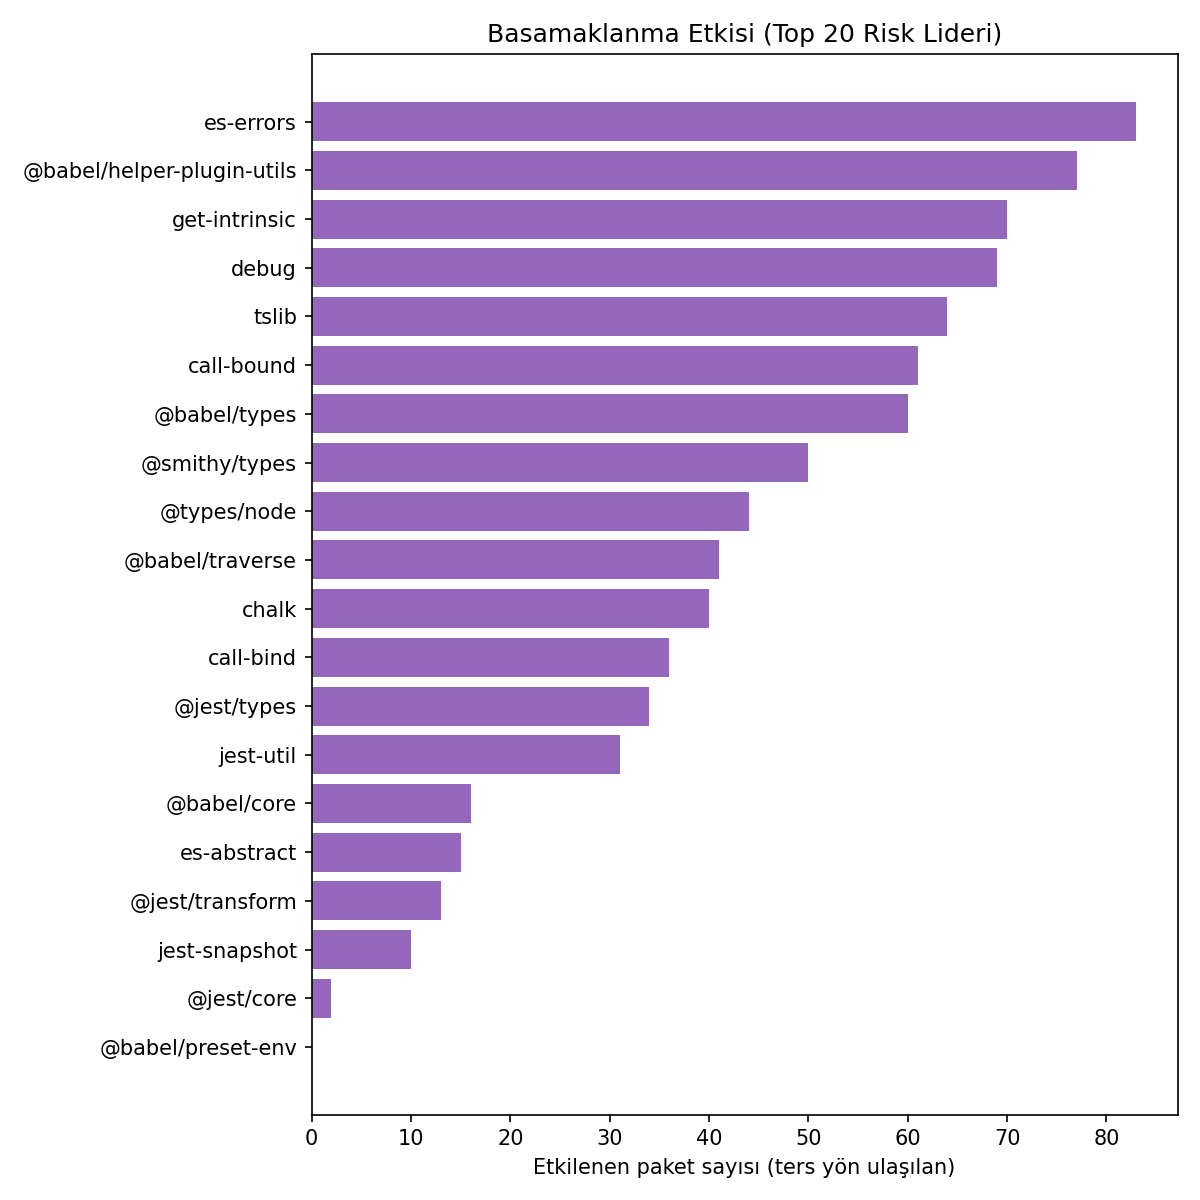
\includegraphics{cascade_impact_top20.png}
  \caption{Risk skoruna göre en riskli 20 paket için kaskad etki büyüklüğü. Yüksek risk genellikle daha büyük kaskada karşılık gelse de, topolojiye bağlı istisnalar görülebilir.}
\end{figure}
\IfFileExists{../results/cascade_impact_top20.tex}{\begin{table}[h]
\centering
\caption{Basamaklanma Etkisi: Top 20 (Ters y"onde etkilenebilecek paket say\i s\i)}
\begin{tabular}{l r}
\toprule
Paket & Etkilenen Paket Say\i s\i \\ \midrule
es-errors & 83 \
@babel/helper-plugin-utils & 77 \
get-intrinsic & 70 \
debug & 69 \
tslib & 64 \
call-bound & 61 \
@babel/types & 60 \
@smithy/types & 50 \
@types/node & 44 \
@babel/traverse & 41 \
chalk & 40 \
call-bind & 36 \
@jest/types & 34 \
jest-util & 31 \
@babel/core & 16 \
es-abstract & 15 \
@jest/transform & 13 \
jest-snapshot & 10 \
@jest/core & 2 \
@babel/preset-env & 0 \
\bottomrule
\end{tabular}
\end{table}
}{\fbox{cascade\_impact\_top20.tex bulunamadı}}

\begin{figure}[H]
  \centering
  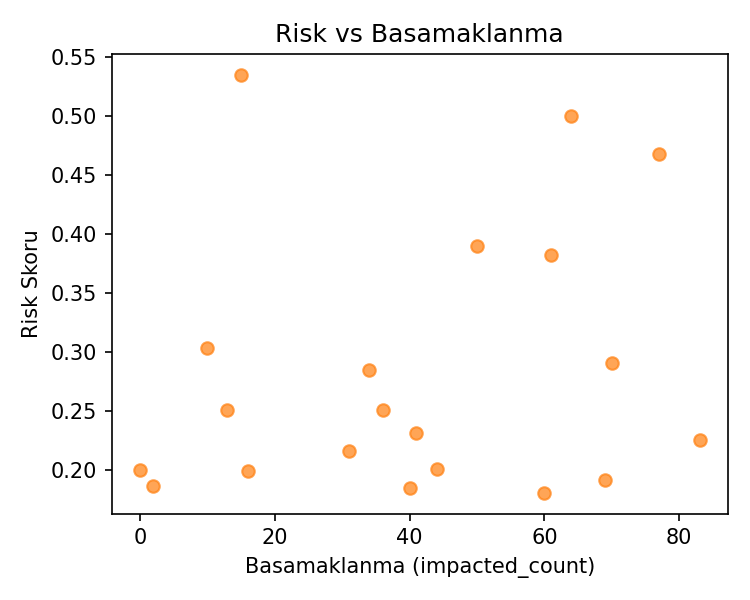
\includegraphics{risk_vs_cascade.png}
  \caption{Risk skoru ile kaskad etkisi ilişkisi (saçılım grafiği). Doğrusal olmayan yapı, tek başına derece metriklerinin tüm \emph{yayılım dinamiğini} açıklamadığını gösterir.}
\end{figure}

\noindent Kaskad etkisi, ağın bağlantı yapısına duyarlıdır: Aynı risk puanına sahip iki düğüm, komşuluklarının farklılığı nedeniyle farklı kaskad profilleri üretebilir.

\subsection{Köprü Kenarlar}
\noindent En yüksek \emph{edge betweenness} değerine sahip kenarlar, alt-ağlar arasında \emph{kırılgan} bağlantıları işaret eder; bu kenarlar üzerindeki trafik, topolojik ayrışma noktalarını anlamaya yardımcı olur.
\IfFileExists{../results/edge_betweenness_top10.tex}{\begin{longtable}{l l r}
\caption{Edge Betweenness Ilk 10 (Yuksek kopru kenarlar)}\\
\toprule
U & V & Edge Betweenness \\
\midrule
\endfirsthead
\toprule
U & V & Edge Betweenness \\
\midrule
\endhead
\bottomrule
\endfoot
\bottomrule
\endlastfoot
@jest/transform & babel-plugin-istanbul & 0.000222 \\
@jest/expect & jest-snapshot & 0.000212 \\
jest-snapshot & @jest/transform & 0.000206 \\
jest & @jest/core & 0.000150 \\
call-bound & get-intrinsic & 0.000150 \\
glob & jackspeak & 0.000147 \\
reflect.getprototypeof & which-builtin-type & 0.000146 \\
jackspeak & @isaacs/cliui & 0.000140 \\
babel-plugin-istanbul & test-exclude & 0.000139 \\
@babel/core & @babel/helper-compilation-targets & 0.000138 \\
\end{longtable}
}{\fbox{edge\_betweenness\_top10.tex bulunamadı}}

\subsection{Ağın Temel İstatistikleri}
\IfFileExists{../results/graph_stats.tex}{\begin{longtable}{l r}
\caption{Graf İstatistikleri (özet)}\\
\toprule
Ölçüt & Değer \\
\midrule
\endfirsthead
\toprule
Ölçüt & Değer \\
\midrule
\endhead
\bottomrule
\endfoot
\bottomrule
\endlastfoot
\textbf{Düğüm sayısı} & 1139 \\
\textbf{Kenar sayısı} & 2164 \\
\textbf{Bileşen sayısı (zayıf)} & 160 \\
\textbf{En büyük bileşen boyutu} & 853 \\
Ortalama in-degree & 1.8999 \\
Ortalama out-degree & 1.8999 \\
\end{longtable}

}{\fbox{graph\_stats.tex bulunamadı}}

\noindent Bu özet tabloda düğüm/kenar sayıları, zayıf bağlanırlık bileşen sayısı, en büyük bileşen boyutu ve ortalama dereceler raporlanır. \emph{Zayıf} (weak) bileşen, kenar yönleri yok sayıldığında bağlı olan düğüm kümeleridir; \emph{güçlü} (strong) bileşen, her düğüm çiftinin birbirine yönlü yollarla erişebildiği alt-kümedir (bu raporda zayıf bileşenler kullanılmıştır).

\subsection{Ana Bulgular }
\begin{itemize}
  \item Ağ ağır kuyrukludur: Az sayıda yüksek etkili \emph{omurga} paket ve çok sayıda düşük dereceli paket birlikte bulunur.
  \item In-degree ve betweenness çoğu zaman birlikte yükselir: Omurga paketler aynı zamanda \emph{köprü} rolü oynar.
  \item Yüksek out-degree, geniş bağımlılık yüzeyi ve artan maruziyeti işaret eder; bu paketler tedarik riski açısından duyarlıdır.
  \item Bileşik risk skoru, tekil metriklerin sınırlamalarını dengeleyerek \emph{karşılaştırılabilir} bir sıralama sağlar.
  \item Kritik düğümlerin çıkarılması, bileşenleşmeyi hızlandırır ve en büyük bileşenin küçülmesine yol açar: Ağ, kritik düğüm kaybına duyarlıdır.
\end{itemize}

\section{Sınırlamalar}
\textbf{Veri.} Varsayılan olarak yalnızca dependencies alanı kullanılmıştır; peerDependencies isteğe bağlıdır. Global dependent sayıları doğrudan dahil edilmemiştir. API kaynaklı eksiklikler ve isimlendirme farklılıkları ölçümleri etkileyebilir.

\textbf{Modelleme.} Betweenness büyük graflarda örnekleme ile hesaplanmıştır; yakınsama, ağ büyüklüğü ve $k$ seçimine bağlıdır. Min--max normalizasyonu gözlenen aralığa bağımlıdır; sıra korunsa da mutlak değerlerin yorumu veri setine özeldir.

\textbf{Sunum.} Ağ görselleri büyük dosyalardır; çizim sıralaması ve düzen parametreleri, yerleşim sezgisellerine (layout) bağlı görsel yanlılıklar taşıyabilir.

\section{Sonuç}
NPM ekosistemi, az sayıda \emph{omurga} ve \emph{köprü} paket etrafında yoğunlaşan bir topoloji sergiler. Bileşik risk skoru ve sağlamlık bulguları, tedarik zinciri güvenliğinde \emph{yapısal} bakışın analitik değerini açıkça ortaya koyar: Kritik paketlerin izlenmesi ve korunması, geniş ölçekli kaskad etkilerini sınırlamada belirleyicidir.

\paragraph{Tekrarlanabilirlik.} Tüm kod ve çıktı üretimi depo içindedir. \texttt{analysis.ipynb} çalıştırılarak results/ çıktıları yeniden üretilebilir ve bu makale derlenebilir.

\end{document}

